%----------------------------------------------------------------------------------------
%	SECTION 1.2
%----------------------------------------------------------------------------------------

\section{The Basis and Subbasis for a Topology.}

\begin{definition}
    If $X$ is a set, the \textbf{basis} for a topology on $X$ is a collection $\Bc$ of 
    subsets of  $X$, called \textbf{basis elements}, such that:
        \begin{enumerate}[label=(\arabic*)]
            \item For every $x \in X$, there is a  $B \in \Bc$ such that $x \in B$.

            \item For $B_1,B_2 \in \Bc$, if $x \in B_1 \cap B_2$, then there is a $B_3 \in \Bc$ 
                such that $x \in B_3 \subseteq B_1 \cap B_2$
        \end{enumerate}
We define the topology $\Tc$ \textbf{generated} by $\Bc$ to be collection of open sets: 
$\Tc=\{U \subseteq X: x \in B \text{ for some } B \in \Bc\}$.
\end{definition}

\begin{theorem}\label{1.2.1}
    Let $X$ be a set, and  $\Bc$ a basis of  $X$, then the collection of subsets 
    of  $X$, $\Tc=\{U \subseteq X: x \in B \text{ for some } B \in \Bc\}$ is a topology on $X$.
\end{theorem}
\begin{proof}
    Let $\Bc$ be a basis for a topology in  $X$, and consider  $\Tc$ as defined 
    above. Cleary, $\emptyset \in X$ and so is  $X$.

    Now let  $\{U_{\alpha}\}$ be a subcollection of subsets of  $X$, and let  $U=\bigcup{U_{\alpha}}$. 
    Then if  $x \in U$ for some  $\alpha$, there is a  $B_{\alpha}$ such that  $x \in B_{\alpha} \subseteq U_{\alpha}$, 
    thus  $x \in B_{\alpha} \subseteq U$.

    Now let  $x \in  U_1 \cap U_2$, and choose $B_1,B_2 \in \Bc$ such that $x \in B_1 \subseteq U_1$ 
    and $x \in B_2 \subseteq U_2$. Then  by definition, there is a $B_3$ for which $x \in B_3 \subseteq B_1 \cap B_2$.
    Now suppose for arbitrary $n$, that  $U=\bigcap_{i=1}^{n}{U_i} \in \Tc$, for some finite 
    subcollection  $\{U_i\}$ of subsets of  $X$. Then by let  $B_n, B_{n+1} \in \Bc$ such that 
    $x \in B_n \subseteq U$ and  $x \in B_{n+1} \subseteq U_{n+1}$. Then by our hypothesis, there is a  $B$ 
for which  $x \in B \subseteq B_n \cap B_{n+1}$, thus  $U \cap U_{n+1}=\bigcap_{i=1}^{n+1}{U_i} \in \Tc$. 
This make $\Tc$ a topology on  $X$.
\end{proof}

\begin{example}
    \begin{enumerate}[label=(\arabic*)]
        \item Let $\Bc$ be the set of all circular regions in the plane  $\R \times \R$, then 
            $\Bc$ satisfies the conditions needed for a basis.

        \item The collection  $\Bc'$ in  $\R \times \R$ of all rectangular region also 
            forms a basis for a topology on  $\R \times \R$.

        \item For any set  $X$, the set of all  $1$-point elements of  $X$ forms a 
            basis for a topology on  $X$.
    \end{enumerate}		
\end{example}

\begin{figure}
    \centering
    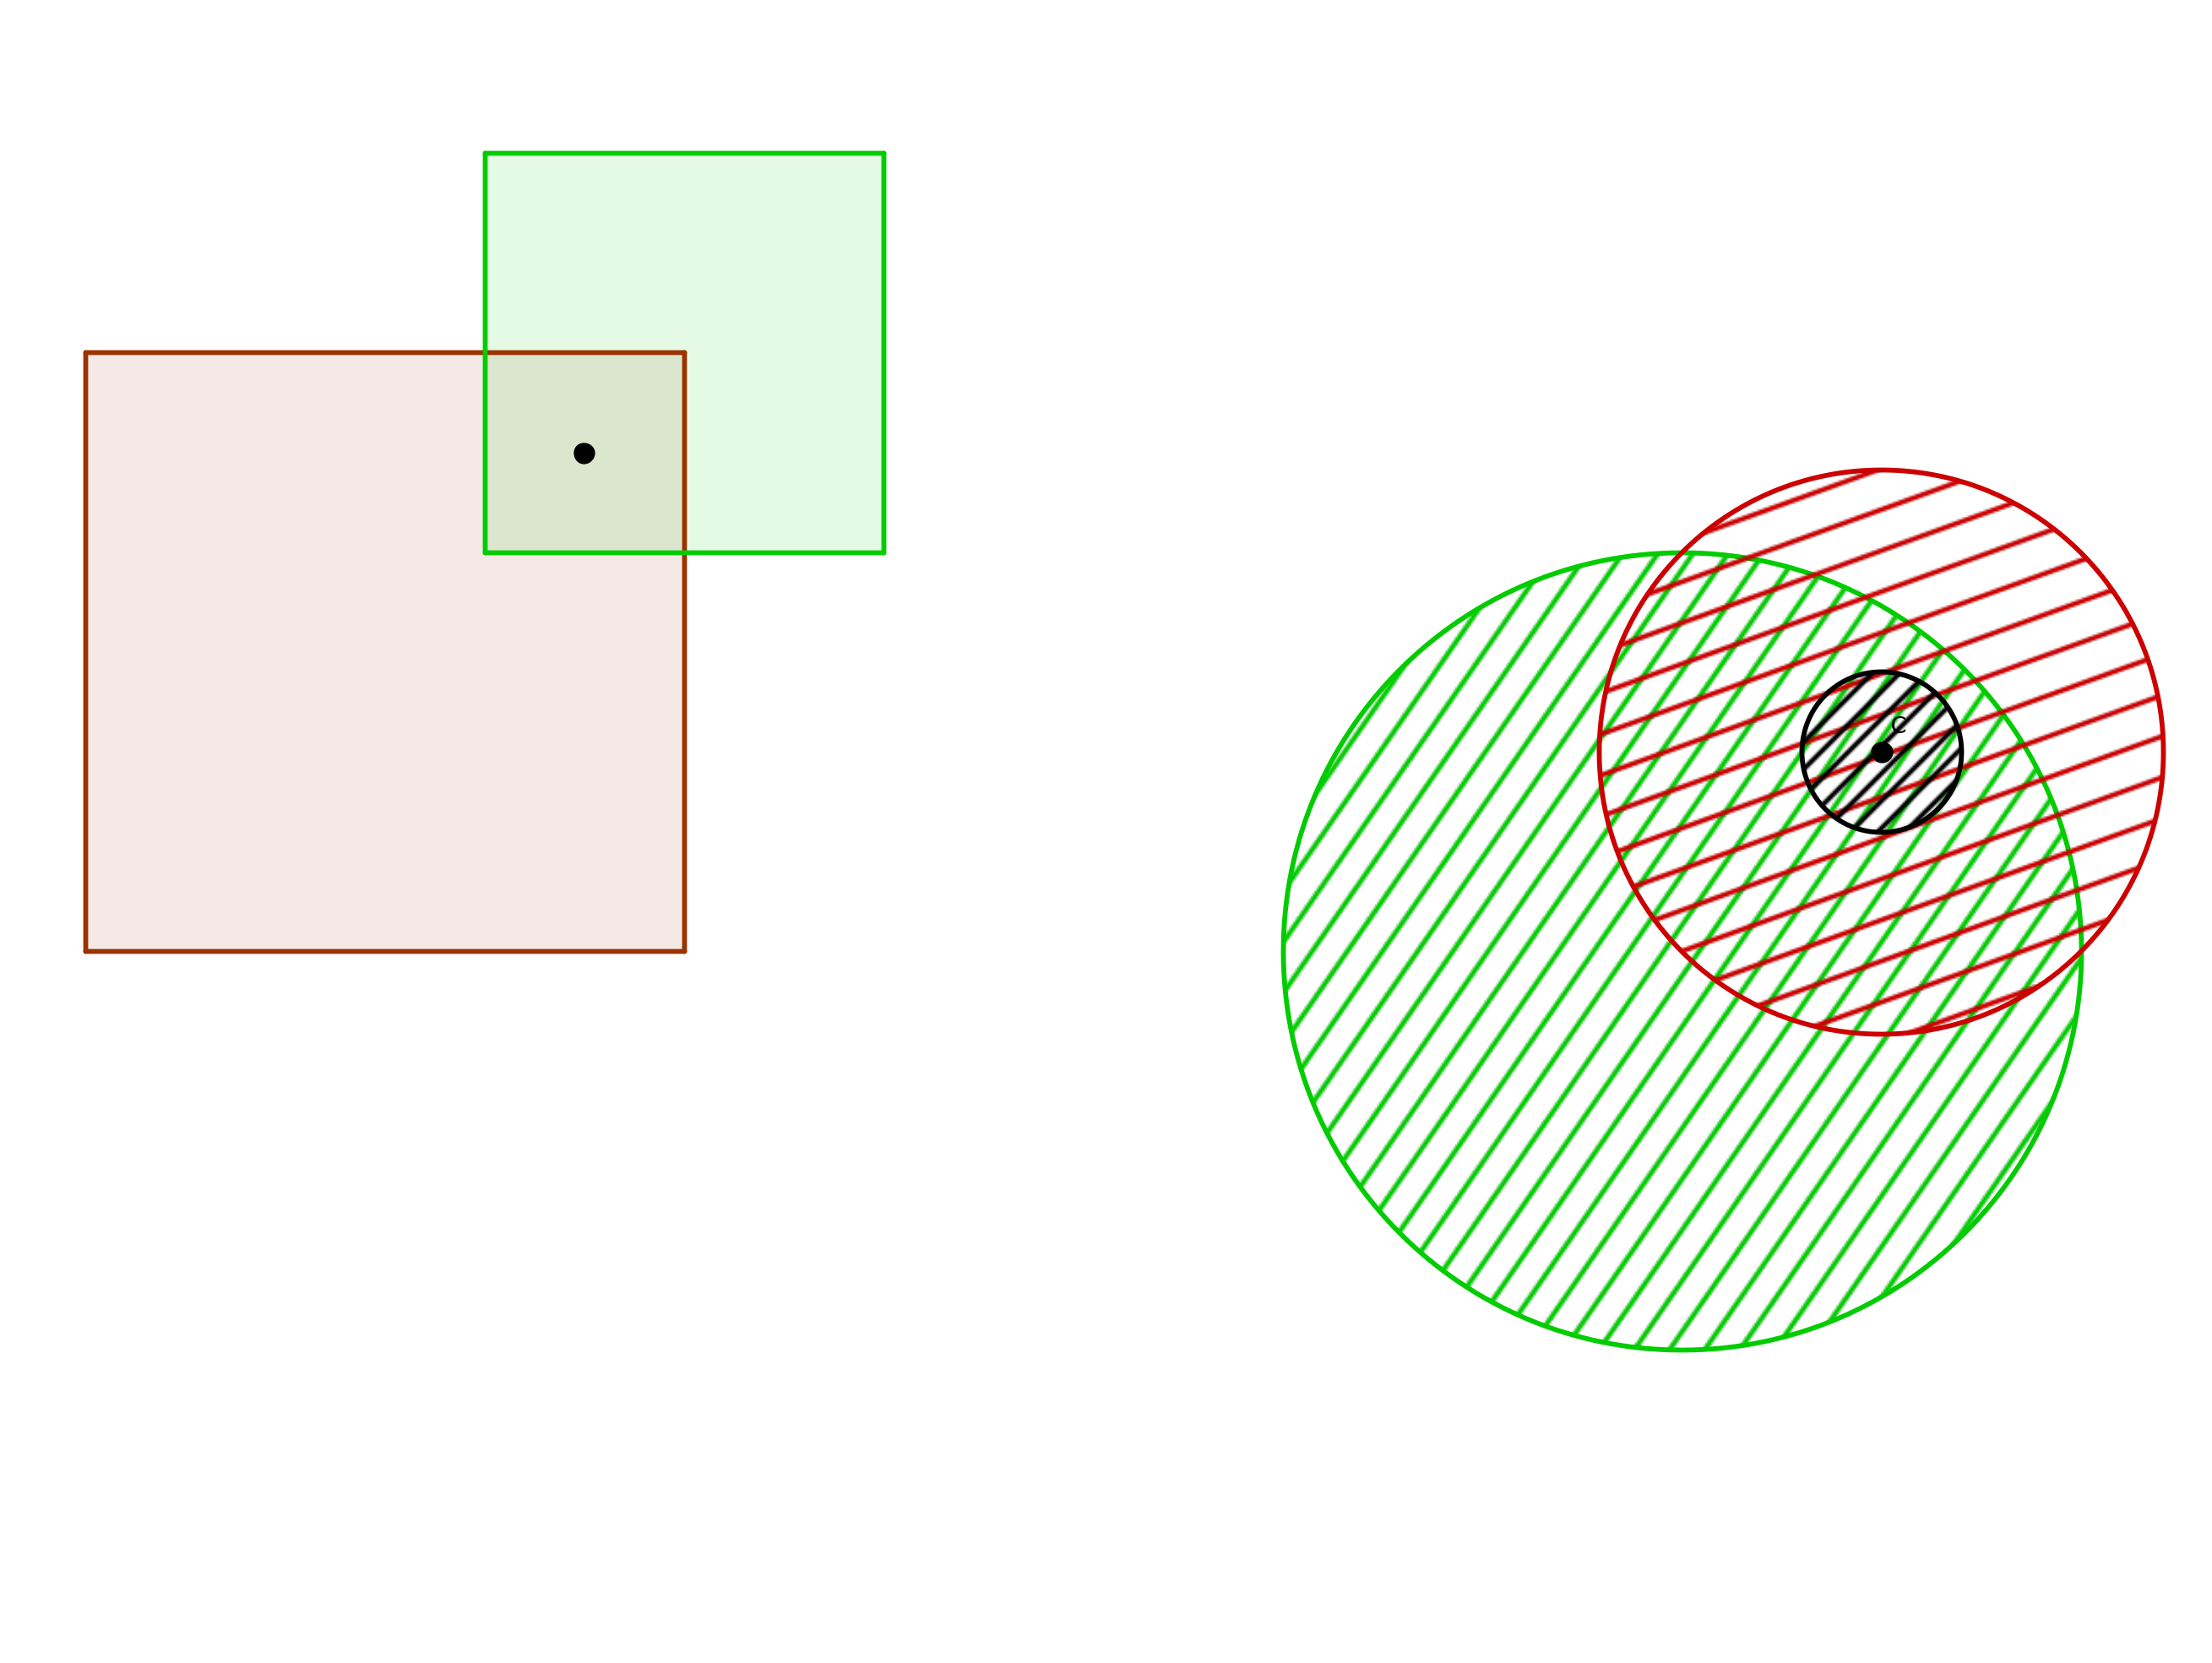
\includegraphics[scale = 0.3]{Figures/Chapter1/basesOfCircularRectangularRegions.png}
    \caption{The basis for $\Bc$ and  $\Bc'$ in  $\R \times \R$  (see example $(2)$).}
    \label{fig_1.2}
\end{figure}

\begin{lemma}\label{1.2.2}
    Let $X$ be a set, and  $\Bc$ be a basis for a topology  $\Tc$ on  $X$. Then 
    $\Tc=\{\bigcup{B}: B \in \Bc\}$.
\end{lemma}
\begin{proof}
    Given a collection $\{B\}$ of basis elements in  $\Bc$, since they are all in  $\Tc$, 
    their unions are also in $\Tc$. Conversely, given  $U \in \Tc$, then for every point 
    $x \in U$, choose a  $B_x \in \B_x$ such that  $x \in B_x \subseteq U$, then  $U=\bigcup_{x \in U}{B_x}$.
\end{proof}
